\chapter{Genetic Algorithm: Validation, Results and Comparison with SA}
\label{ch:garesults}

This chapter documents the \ac{GA} case studies and inputs (Section~\ref{sec:gacases}), its generic
validation (Section~\ref{sec:gavalid}), the parameter study that fixed the settings of
Table~\ref{tab:gaparams} (Section~\ref{sec:gaparamstudy}), the results of the case studies
(Section~\ref{sec:gacaseresults}), the harder tests (Section~\ref{sec:gahard}), the comparison with
\ac{SA} on the nine case studies (Section~\ref{sec:sa-vs-ga}) and a matched comparison on a larger
Eros case (Section~\ref{sec:garesults}). Every run is produced by \texttt{experiments/validate.py}
(parts G2, GV4, GV5, GP, H, B, M and NI) and the report assets by \texttt{experiments/ga\_assets.py}.

%=====================================================================================
\section{Case studies and input parameters}
\label{sec:gacases}

The \ac{GA} is run on the nine case studies A1--A6 and B1--B3 of Table~\ref{tab:cases}, with the
\emph{same} evaluation budget (2000), the \emph{same} random seeds (0--4) and the same mission
settings as \ac{SA}, so that every \ac{GA} run has an \ac{SA} twin. Three new cases push the problem
to its limits: the large body Kleopatra with very short missions, and a fleet of up to 20 spacecraft
(101 genes, twice the largest case of Milestone~3). A fourth series repeats three cases with a budget
of 5000 evaluations, and case M compares both algorithms once more on a ten-day Eros mission with
ten slots and a finer search mesh. Table~\ref{tab:gacases} lists the new cases; all \ac{GA}
parameters are those of Table~\ref{tab:gaparams}.

\begin{table}[htbp]
\centering
\caption{Additional case studies of this milestone (mission settings as in Table~\ref{tab:cases};
$T_{\min}=\min(6\,\mathrm{h},T_{\max}/4)$; five seeds per algorithm, three for case M).}
\label{tab:gacases}
\footnotesize
\begin{tabularx}{\textwidth}{@{}p{0.6cm}p{2.6cm}p{0.8cm}p{0.8cm}p{0.7cm}p{0.6cm}p{1.2cm}X@{}}
\toprule
Case & Body, setting & $T_{\max}$ & $T_{\min}$ & $N_{\max}$ & dim & Budget & Question \\
\midrule
H1 & Kleopatra & 6 h & 1.5 h & 10 & 51 & 2000 & \multirow{3}{=}{The hardest missions: a 219\,km body with a few hours, up to 101 genes. Which algorithm copes better?} \\
H2 & Kleopatra & 2 h & 0.5 h & 10 & 51 & 2000 & \\
H3 & Kleopatra & 6 h & 1.5 h & 20 & 101 & 2000 & \\
\midrule
L1 & Eros (= A2) & 1 d & 6 h & 5 & 26 & 5000 & \multirow{3}{=}{Does a larger budget change the ranking of the two algorithms?} \\
L2 & Eros (= A6) & 2 h & 0.5 h & 10 & 51 & 5000 & \\
L3 & Kleopatra (= B3) & 12 h & 3 h & 10 & 51 & 5000 & \\
\midrule
F & Eros, GA parameters varied & 2 d & 6 h & 5 & 26 & 2000 & parameter study (same case as \ac{SA}'s case E) \\
\midrule
M & Eros, 3\,000-facet mesh & 10 d & 6 h & 10 & 51 & 1200 & matched comparison, seeds 0--2 (Section~\ref{sec:garesults}) \\
\bottomrule
\end{tabularx}
\end{table}

Cases H1--H3 are also solved by random search. Case F changes one \ac{GA} parameter at a time from
the defaults (23 settings, Table~\ref{tab:gaparams}).

%=====================================================================================
\section{Validation}
\label{sec:gavalid}

\paragraph{Known optima (G2).} Since the \ac{GA} only sees the \texttt{Problem} interface, it is run
unchanged on the benchmark functions of validation V2, whose global minimum is 0 at $\mathbf{x}=0$
(10 seeds, 10\,000 evaluations each; Section~\ref{sec:ga-generic}: without slots, every gene is its
own group). Table~\ref{tab:g2} compares it with \ac{SA}. The \ac{GA} reaches the optimum in every
run of every function, with mean errors between $10^{-9}$ and $10^{-3}$ (at most $2\cdot10^{-3}$ in any run), several orders of magnitude
below those of \ac{SA}. On the five-dimensional Rastrigin function, which has about $10^5$ local
minima, \ac{SA} ends below 0.1 in only 70\,\% of the runs and the \ac{GA} in all of them: the
population and the recombination of good coordinates from different individuals are exactly what
a separable, highly multimodal function rewards. This validates the selection, elitism, crossover,
mutation and budget machinery independently of the spacecraft model.

\begin{table}[htbp]
\centering
\caption{Known-optimum test (minimum 0): best value reached, 10 seeds $\times$ 10\,000 evaluations.}
\label{tab:g2}
\small
\begin{tabular}{@{}lcccccc@{}}
\toprule
 & & \multicolumn{2}{c}{mean best value} & \multicolumn{2}{c}{worst run} & runs below 0.1 \\
\cmidrule(lr){3-4}\cmidrule(lr){5-6}
Function & $n$ & SA & GA & SA & GA & SA / GA \\
\midrule
Sphere & 5 & 2.5e-03 & 6.8e-10 & 4.0e-03 & 6.1e-09 & 100 / 100\,\% \\
Rastrigin & 2 & 2.1e-02 & 1.8e-08 & 1.2e-01 & 1.5e-07 & 90 / 100\,\% \\
Rastrigin & 5 & 4.7e-01 & 3.9e-07 & 2.0e+00 & 2.3e-06 & 70 / 100\,\% \\
Ackley & 2 & 1.2e-02 & 1.1e-04 & 2.4e-02 & 3.2e-04 & 100 / 100\,\% \\
Ackley & 5 & 1.9e-02 & 3.2e-04 & 3.5e-02 & 1.9e-03 & 100 / 100\,\% \\
\bottomrule
\end{tabular}

\end{table}

\paragraph{Comparison with the literature (GV5).} Under the assumptions of the literature (every
facet lit, no shadows; case D of Table~\ref{tab:cases}) the \ac{GA} images on average
\gaAllLitC\,\% (best \gaAllLitBestC\,\%) of Eros, against 97.9\,\% for \ac{SA} (case D) and the
100\,\% that Nallapu and Thangavelautham~\cite{nallapu2019} report with a simpler visibility model
(validation V5). Both algorithms choose two spacecraft and a
mission of about 1.16 days, and their fitness is the same within 0.5\,\% ($J=0.0730$ for the \ac{GA},
$0.0733$ for \ac{SA}).

\paragraph{Feasibility and finer model.} All \gaFeasible{} final \ac{GA} designs of the case studies
are feasible. Re-evaluated on the four times finer shape model (6000 facets), the coverage of the
30 Eros designs changes by 2.0 points on average (at most 2.9), the same accuracy as found for the
\ac{SA} designs in validation V7: the \ac{GA} does not exploit the coarseness of the search model.

%=====================================================================================
\section{Parameter study}
\label{sec:gaparamstudy}

Case F changes one parameter at a time from the starting values of Table~\ref{tab:gaparams}
(five seeds each). Figure~\ref{fig:gaparams} shows every run and Table~\ref{tab:gp} the statistics.
A value was to replace the starting value only if it was better by more than the seed-to-seed
spread; a one-sided Mann--Whitney test~\cite{mann1947} against the default decides.

\begin{figure}[htbp]
\centering
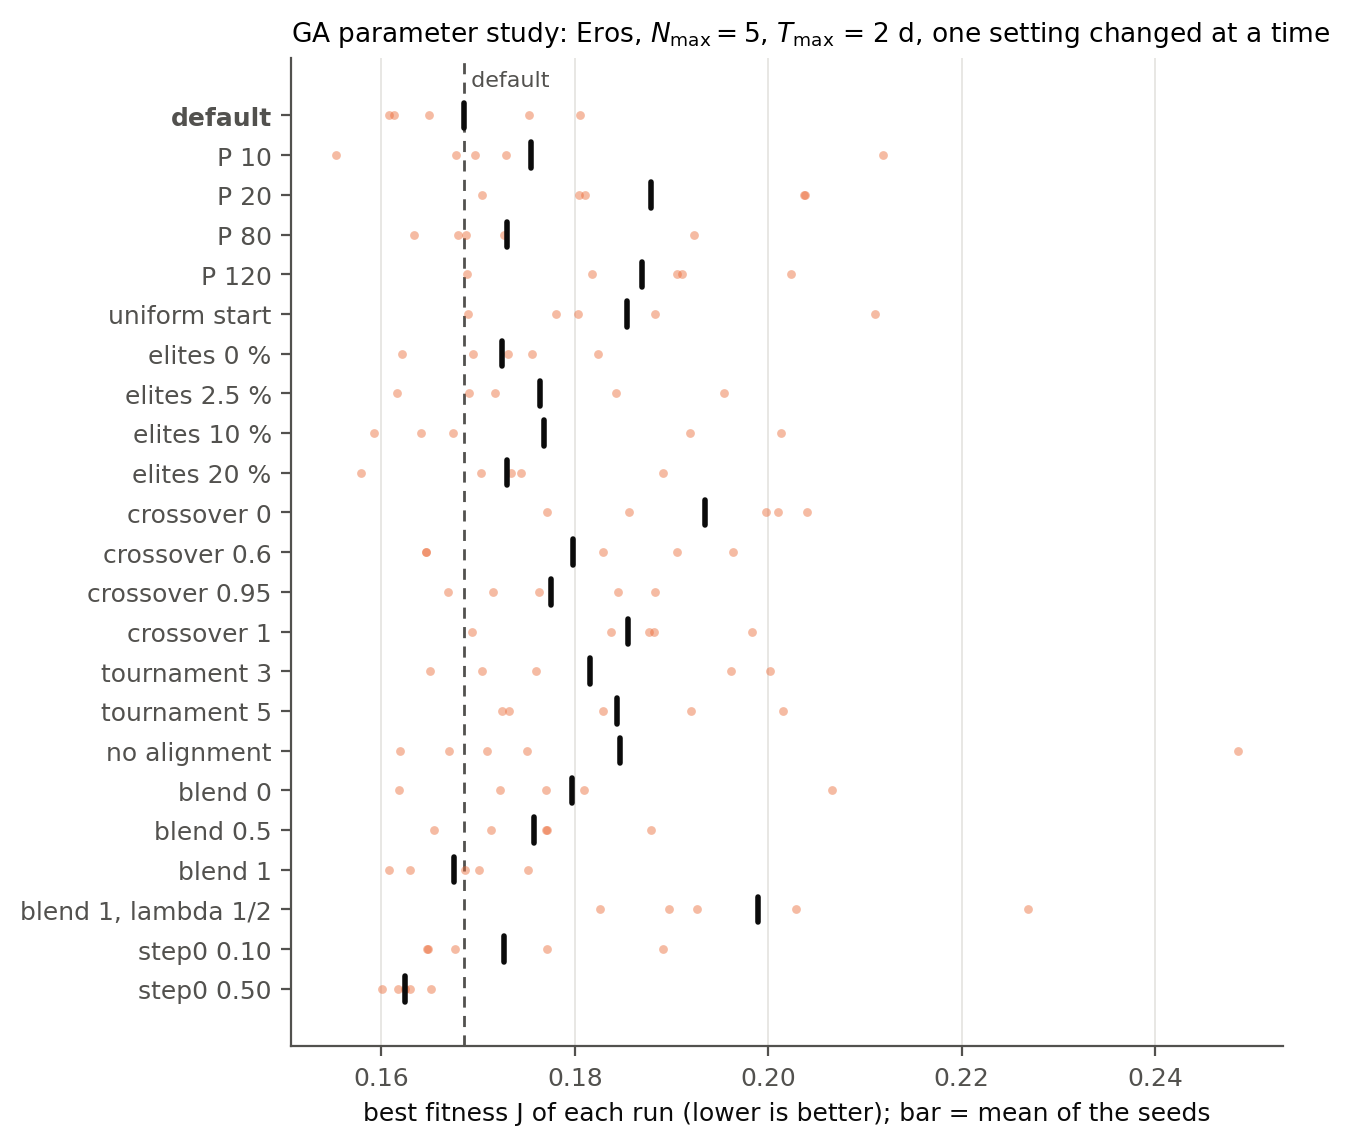
\includegraphics[width=0.86\textwidth]{Figures/fig_ga_params.png}
\caption{Parameter study of the \ac{GA} (case F). Dots: best design of each of the five runs; bar:
mean. Dashed line: the default settings.}
\label{fig:gaparams}
\end{figure}

\begin{table}[htbp]
\centering
\caption{Parameter study (case F, five seeds per setting). Tracks: spacecraft actually simulated per
run (computing cost independent of the machine).}
\label{tab:gp}
\footnotesize
\begin{tabular}{@{}lcccccc@{}}
\toprule
Setting & mean $J$ & std $J$ & best $J$ & mean $C$ [\%] & mean $N$ & tracks / run \\
\midrule
\textbf{default} & 0.1685 & 0.0089 & 0.1608 & 92.7 & 3.0 & 1946 \\
P 10 & 0.1755 & 0.0214 & 0.1553 & 92.3 & 2.8 & 1732 \\
P 20 & 0.1879 & 0.0151 & 0.1704 & 93.4 & 3.0 & 1832 \\
P 80 & 0.1730 & 0.0113 & 0.1633 & 93.3 & 3.0 & 1990 \\
P 120 & 0.1869 & 0.0125 & 0.1689 & 90.4 & 3.2 & 2173 \\
uniform start & 0.1854 & 0.0159 & 0.1690 & 93.6 & 3.0 & 1784 \\
elites 0 \% & 0.1725 & 0.0075 & 0.1621 & 92.0 & 3.4 & 2061 \\
elites 2.5 \% & 0.1764 & 0.0134 & 0.1617 & 89.6 & 3.0 & 1938 \\
elites 10 \% & 0.1768 & 0.0186 & 0.1593 & 93.7 & 3.0 & 1904 \\
elites 20 \% & 0.1730 & 0.0111 & 0.1579 & 93.7 & 3.2 & 1918 \\
crossover 0 & 0.1935 & 0.0116 & 0.1771 & 89.3 & 3.0 & 2127 \\
crossover 0.6 & 0.1798 & 0.0147 & 0.1646 & 91.2 & 3.0 & 1947 \\
crossover 0.95 & 0.1775 & 0.0089 & 0.1669 & 93.5 & 3.2 & 1826 \\
crossover 1 & 0.1855 & 0.0105 & 0.1694 & 92.0 & 3.2 & 1936 \\
tournament 3 & 0.1815 & 0.0157 & 0.1650 & 92.6 & 3.0 & 1866 \\
tournament 5 & 0.1844 & 0.0125 & 0.1724 & 92.2 & 3.4 & 1894 \\
no alignment & 0.1847 & 0.0360 & 0.1620 & 92.0 & 3.2 & 1917 \\
blend 0 & 0.1797 & 0.0166 & 0.1619 & 89.9 & 3.0 & 897 \\
blend 0.5 & 0.1758 & 0.0083 & 0.1654 & 92.7 & 3.0 & 2895 \\
blend 1 & 0.1676 & 0.0058 & 0.1608 & 92.0 & 2.8 & 5381 \\
blend 1, $\lambda=\frac12$ & 0.1989 & 0.0172 & 0.1826 & 90.1 & 3.2 & 4299 \\
step0 0.10 & 0.1727 & 0.0105 & 0.1647 & 92.5 & 3.2 & 1913 \\
step0 0.50 & \textbf{0.1624} & 0.0019 & 0.1600 & 93.7 & 3.2 & 1925 \\
\bottomrule
\end{tabular}

\end{table}

\begin{itemize}
\item \textbf{No setting is significantly better than the defaults, and seven are significantly
worse} ($p<0.05$): $P=20$, $P=120$, the uniform start, a crossover fraction of 0 or 1, the tournament
size $k=5$ and the fixed blend weight $\lambda=\tfrac12$. The defaults chosen by the reasoning of
Chapter~\ref{ch:ga} are therefore kept.
\item \textbf{Population size:} the expected U-shape. Small populations ($P=10$, 20) lose diversity
early; large ones ($P=120$) leave only about 18 generations for selection and crossover to act.
\item \textbf{Stratified start:} better than the uniform start by 0.017 ($p=0.048$), as argued in
Section~\ref{sec:ga-init}.
\item \textbf{Both operators are needed:} with mutation only ($\chi=0$) the \ac{GA} becomes a set of
\ac{SA}-like steps without \ac{SA}'s acceptance rule and is the second-worst setting; with crossover
only ($\chi=1$) no new gene values can appear. The mixture $\chi=0.8$ is best.
\item \textbf{Blend weight:} the midpoint $\lambda=\tfrac12$ is the worst of all 23 settings
($p=0.004$). It confirms the contraction argument of Section~\ref{sec:ga-crossover}: every blended
gene lies between its parents, the population shrinks and the search stalls.
\item \textbf{Blend probability:} $p_b=1$ reaches the same fitness as $p_b=0.3$ but simulates
2.8 times more spacecraft (5381 against 1946 tracks per run), because every child orbit is new;
$p_b=0$ is the cheapest (897 tracks) but worse. $p_b=0.3$ is the best compromise, as predicted by the
``one new orbit per child'' argument of Table~\ref{tab:pblend}.
\item \textbf{Alignment:} without it the results become erratic (standard deviation four times that
of the default): some runs pair unrelated orbits and fail.
\item \textbf{Mutation step:} $\sigma_0=0.5$ had the best mean over the first five seeds (0.162).
A tie-breaker with ten further seeds (5--14) for both values gave means of 0.1756 ($\sigma_0=0.5$)
and 0.1786 ($\sigma_0=0.25$) over 15 seeds, $p=0.53$: no real difference, so the default is kept. The
tie-breaker also showed that five seeds can be optimistic: the default's mean rose from 0.169 to
0.179. Small differences between good settings in Table~\ref{tab:gp} are therefore within the noise;
only the significant differences are interpreted.
\end{itemize}

%=====================================================================================
\section{Results of the case studies}
\label{sec:gacaseresults}

Figure~\ref{fig:savsga} shows the best design of every run of the nine case studies for the three
algorithms, and Figure~\ref{fig:convsaga} the median convergence. Both optimisers beat random search
by a wide margin in every case and every run. The \ac{GA} reaches 73.5--95.7\,\% coverage on Eros
missions of six hours to ten days and 47.2\,\% in two hours, and 64--76\,\% on Kleopatra.

\begin{figure}[htbp]
\centering
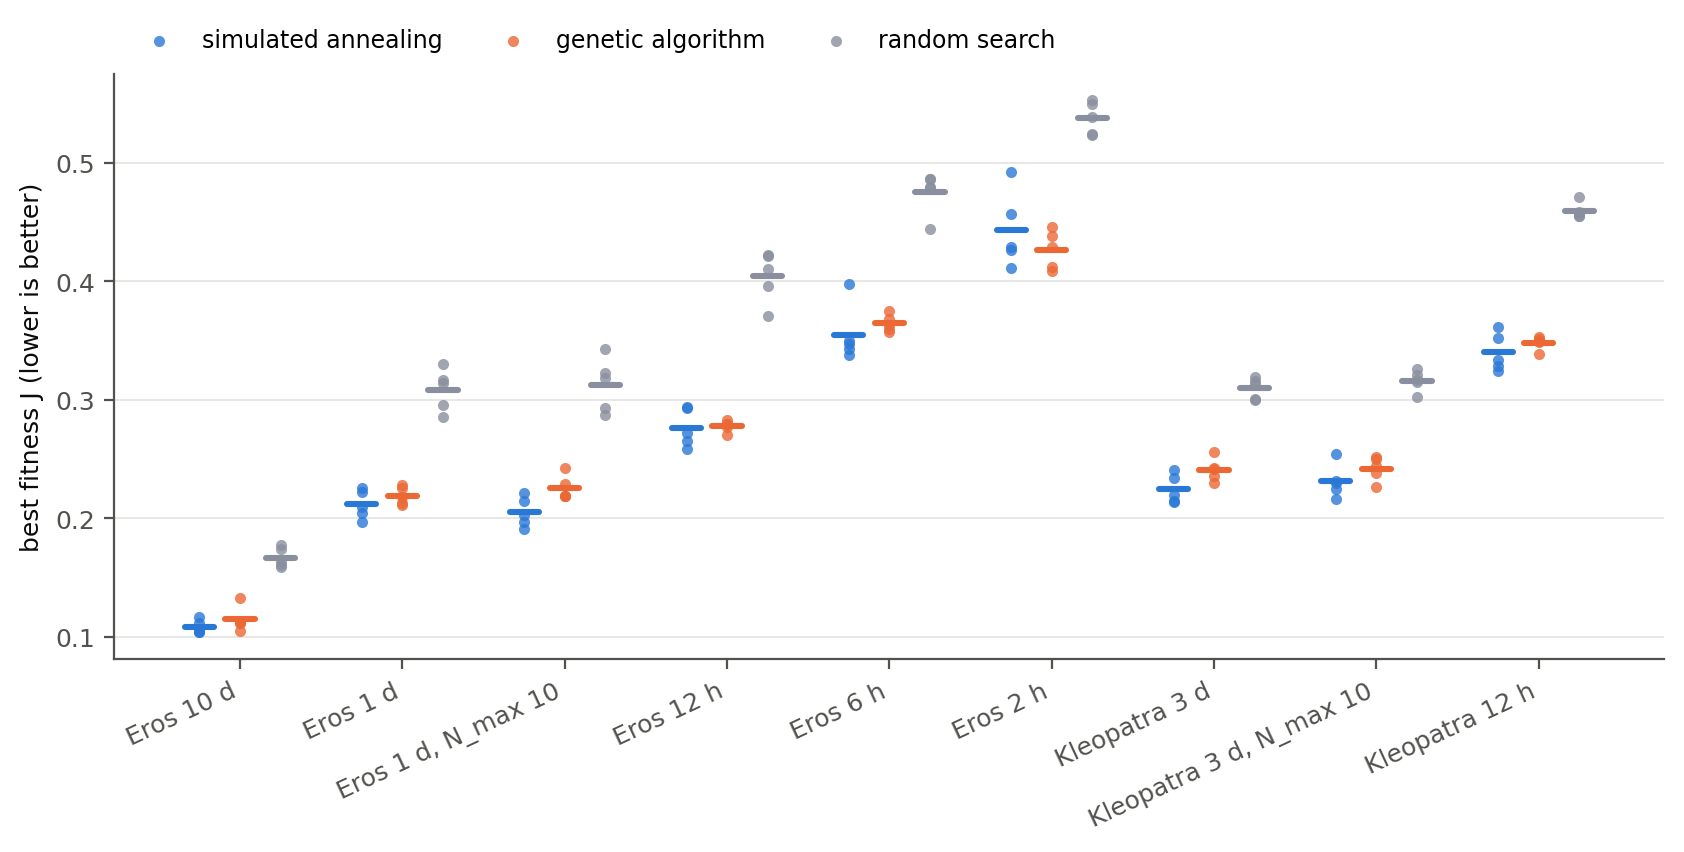
\includegraphics[width=\textwidth]{Figures/fig_sa_vs_ga.png}
\caption{Best fitness of every run (dots) and mean (bar) for \ac{SA}, \ac{GA} and random search,
budget 2000 evaluations, five seeds per algorithm and case.}
\label{fig:savsga}
\end{figure}

\begin{figure}[htbp]
\centering
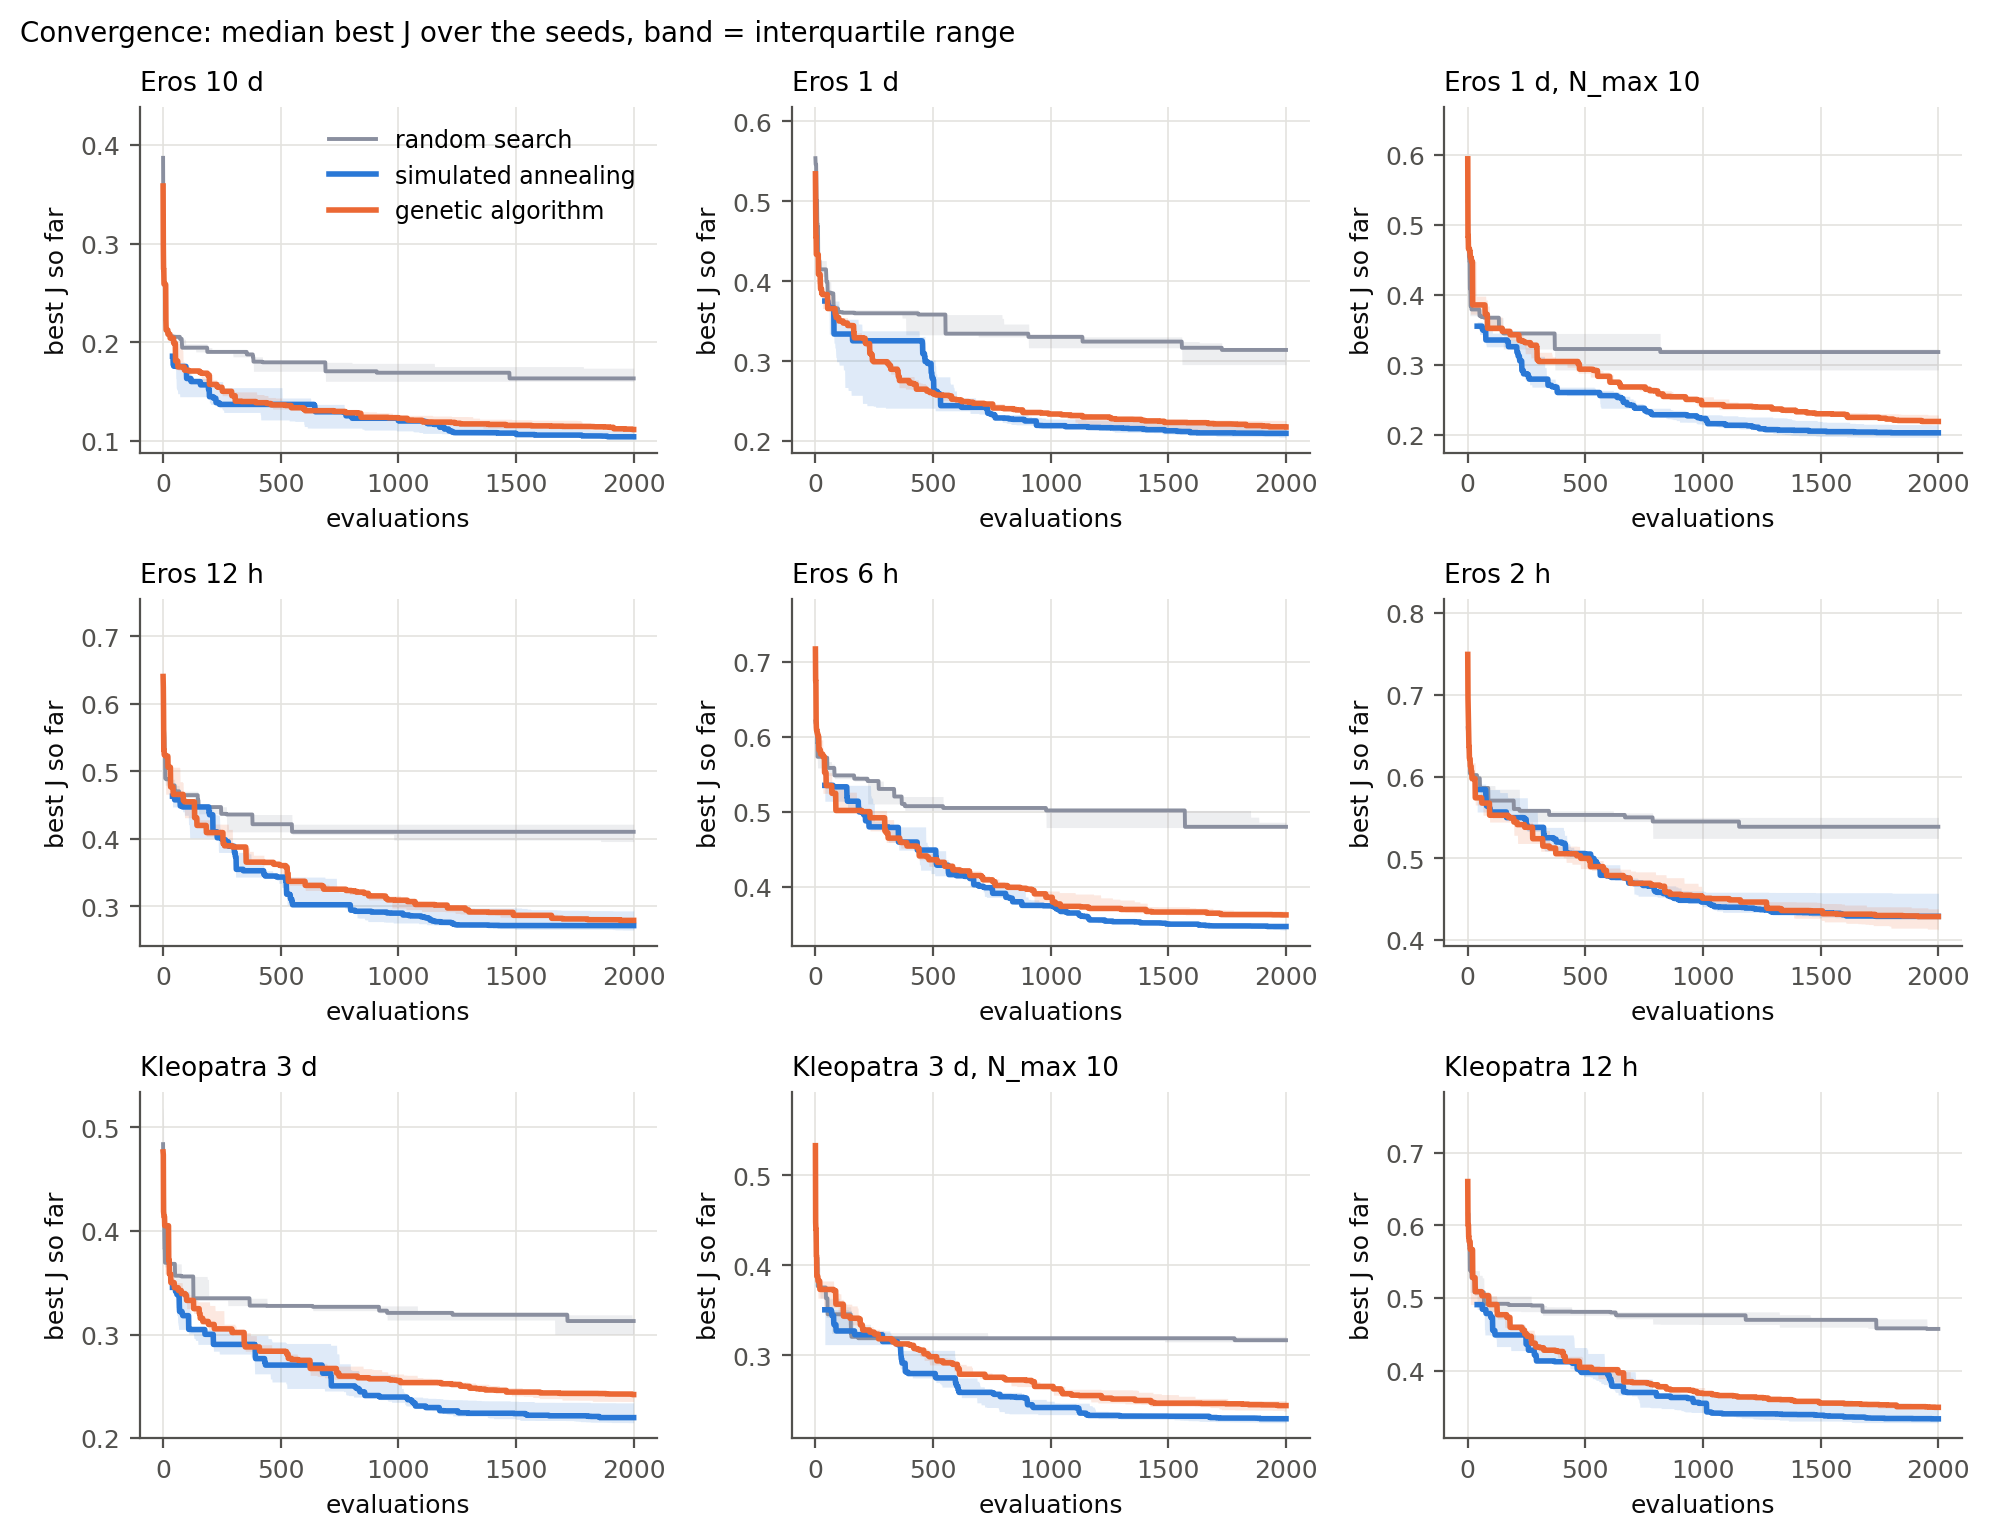
\includegraphics[width=\textwidth]{Figures/fig_convergence_sa_ga.png}
\caption{Convergence: median over the seeds of the best fitness found so far, with the interquartile
band. \ac{SA}'s curve starts after its warm start (the first 40 evaluations are not recorded).}
\label{fig:convsaga}
\end{figure}

\paragraph{Behaviour of one run.} Figure~\ref{fig:gagen} follows the \ac{GA} run with the median
result on Eros 10\,d (case A1). The population mean improves quickly in the first 15
generations (from 0.42 to 0.14), while the diversity of the active genes (their spread as a share of
the range; dormant genes of switched-off slots are not counted) falls from 0.31, the value of a random
population, to about 0.03 after 20 generations: the population concentrates on one region and then
refines it. The fleet sizes in the population stay mixed (two to four spacecraft) for most of the run;
only in the last generations does the population settle on two spacecraft.

\paragraph{Which operator produces the improvements.} Over all 45 case-study runs, the new best
designs came from blend crossover in 73\,\% of the cases, from slot swaps in 18\,\% and from
mutation in 9\,\% (the initial random designs excluded; Figure~\ref{fig:gagen}, right). Although
blending is possible only for pairs of flying slots and is chosen for 30\,\% of them, it is the
operator that \emph{refines} orbits towards the optimum; swaps and mutation supply the combinations
and the new values it works on. This is consistent with the parameter study, in which removing
either the crossover or the mutation group made the \ac{GA} significantly worse.

\begin{figure}[htbp]
\centering
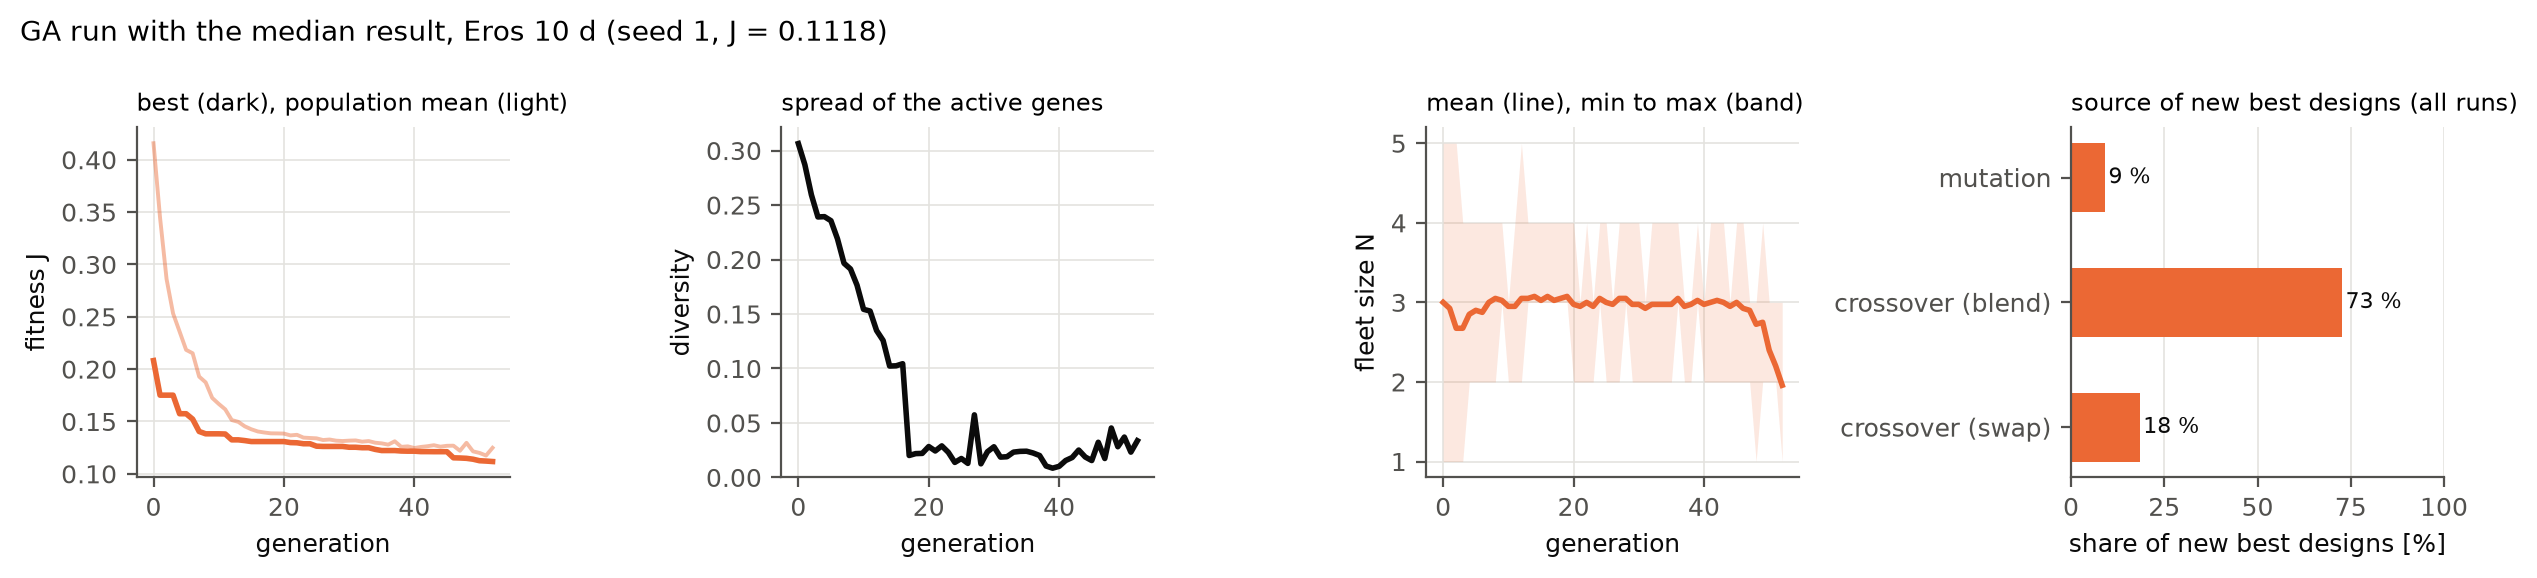
\includegraphics[width=\textwidth]{Figures/fig_ga_generations.png}
\caption{The \ac{GA} run with the median result on Eros 10\,d, generation by generation: fitness,
diversity of the active genes, fleet sizes in the population; right: the operator that produced each
new best design, over all 45 case-study runs.}
\label{fig:gagen}
\end{figure}

%=====================================================================================
\section{Harder tests: large body, short missions, larger budget}
\label{sec:gahard}

\paragraph{Hard cases H1--H3.} Table~\ref{tab:hard} and Figure~\ref{fig:hardbudget} (left) show the
three hardest missions. On the two 10-slot missions H1 and H2 the \ac{GA} has the lower mean fitness
(by 1.5 and 1.3\,\%) and images 5.6 and 7.9 points more of Kleopatra than \ac{SA}, but neither
difference is significant. On the 101-gene case H3 \ac{SA} has the lower mean fitness (0.418 against
0.435; $p=0.11$ for \ac{SA}~$<$~\ac{GA}, not significant), and both algorithms reduce the fleet to three
or four spacecraft in every run, while random search still sends 3 to 8. A first run of H3 used a
cost normalisation $n_{\mathrm{ref}}=\max(10,N)$ that capped $Z$ at one for fleets above ten
spacecraft; under it three \ac{SA} runs stayed at 14--15 spacecraft. With the fixed reference
$n_{\mathrm{ref}}=10$ of the final code (Eq.~\ref{eq:Z}) every extra spacecraft costs
$\Delta Z=0.1$ at any fleet size, and the results above are those of the final code.

\begin{table}[htbp]
\centering
\caption{Hard cases H1--H3 (2000 evaluations, five seeds): mean fitness, coverage and fleet size;
$p$: one-sided Mann--Whitney test that the \ac{GA} is better.}
\label{tab:hard}
\footnotesize
\begin{tabular}{@{}lccccccccc@{}}
\toprule
 & \multicolumn{3}{c}{mean $J$} & \multicolumn{3}{c}{mean $C$ [\%]} & \multicolumn{2}{c}{mean $N$} & \\
\cmidrule(lr){2-4}\cmidrule(lr){5-7}\cmidrule(lr){8-9}
Case & SA & GA & random & SA & GA & random & SA & GA & $p$ (GA $<$ SA) \\
\midrule
Kleopatra 6 h & 0.4408 & 0.4343 & 0.5251 & 39.8 & 45.4 & 30.3 & 2.2 & 3.2 & 0.42 \\
Kleopatra 2 h & 0.4529 & 0.4469 & 0.5325 & 34.3 & 42.2 & 14.9 & 2.6 & 3.6 & 0.50 \\
Kleopatra 6 h, $N_{\max}=$ 20 & 0.4180 & 0.4353 & 0.5686 & 52.2 & 45.7 & 25.9 & 3.4 & 3.6 & 0.92 \\
\bottomrule
\end{tabular}

\end{table}

\paragraph{Larger budget L1--L3.} With 5000 instead of 2000 evaluations both algorithms improve, but
the \ac{GA} 1.6 to 2.9 times more (Table~\ref{tab:budget}, Figure~\ref{fig:hardbudget}, right).
Where \ac{SA} led at 2000 evaluations the gap shrinks from 0.007 to 0.002 (Eros 1\,d) and from
0.008 to 0.005 (Kleopatra 12\,h); on the two-hour Eros mission, where the \ac{GA} already led,
its advantage becomes significant ($p=0.048$).

\begin{table}[htbp]
\centering
\caption{Mean fitness with 2000 and 5000 evaluations (same seeds); $p$: one-sided Mann--Whitney
tests at 5000 evaluations (bold: $p<0.05$).}
\label{tab:budget}
\small
\begin{tabular}{@{}lcccccc@{}}
\toprule
 & \multicolumn{2}{c}{SA mean $J$} & \multicolumn{2}{c}{GA mean $J$} & \multicolumn{2}{c}{$p$ at 5000} \\
\cmidrule(lr){2-3}\cmidrule(lr){4-5}\cmidrule(lr){6-7}
Case & 2000 & 5000 & 2000 & 5000 & GA $<$ SA & SA $<$ GA \\
\midrule
Eros 1 d & 0.2119 & 0.2092 & 0.2191 & 0.2113 & 0.790 & 0.274 \\
Eros 2 h & 0.4432 & 0.4371 & 0.4268 & 0.4133 & \textbf{0.048} & 0.972 \\
Kleopatra 12 h & 0.3403 & 0.3357 & 0.3482 & 0.3410 & 0.845 & 0.210 \\
\bottomrule
\end{tabular}

\end{table}

\begin{figure}[htbp]
\centering
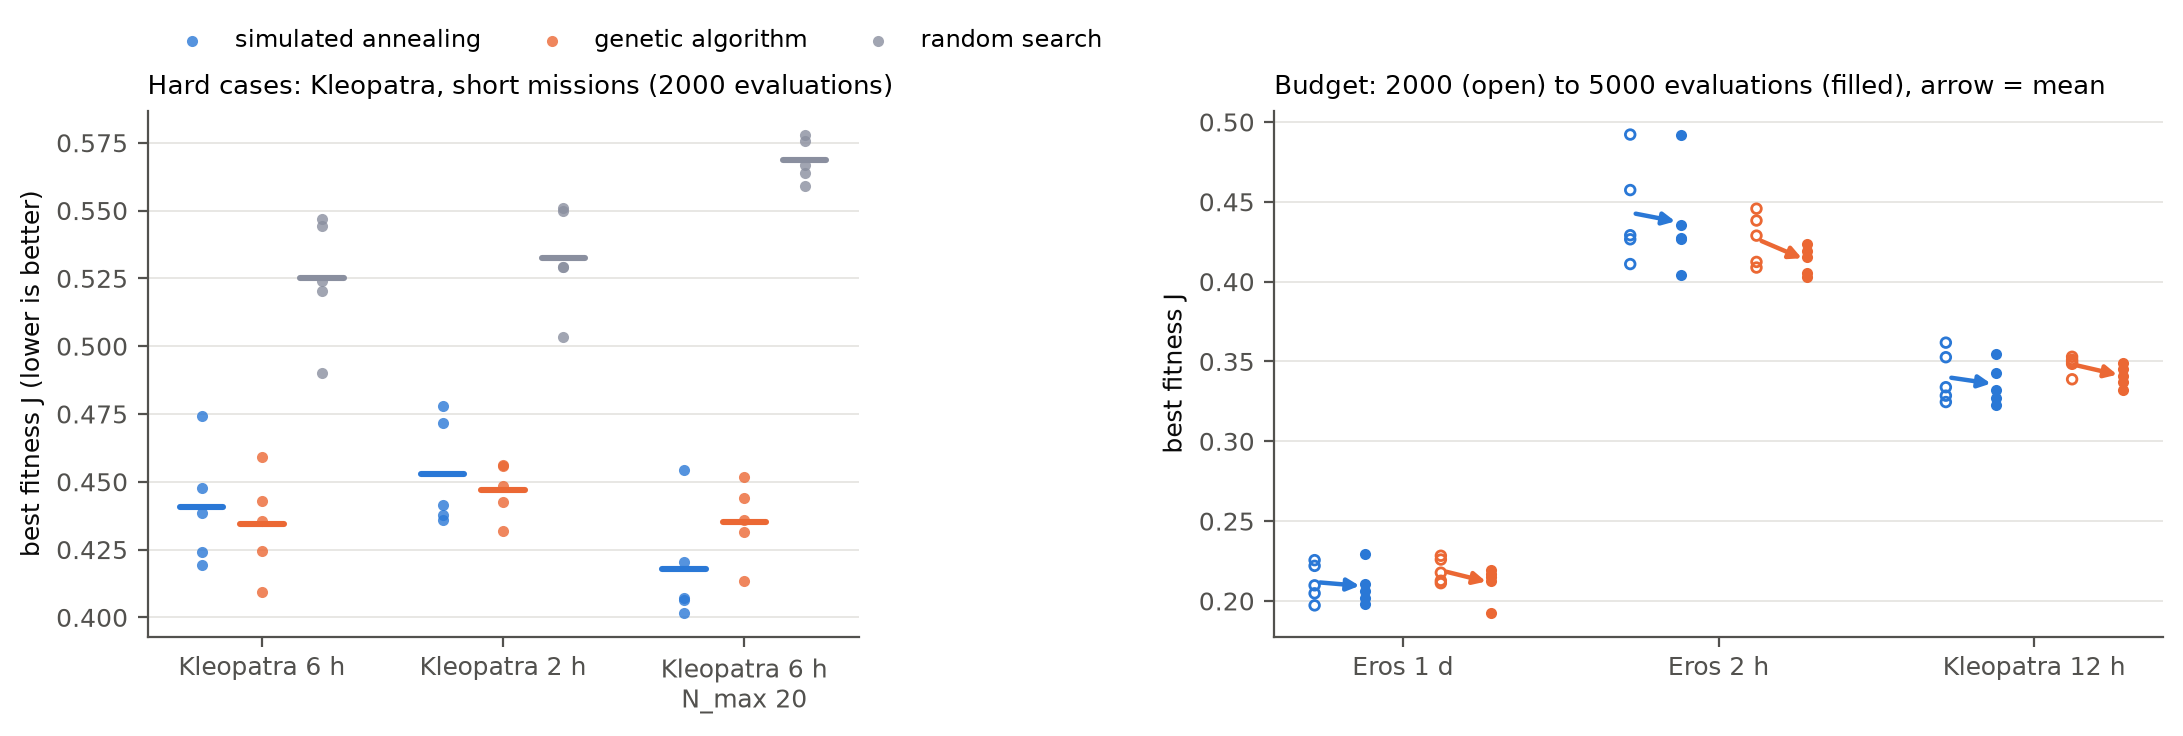
\includegraphics[width=\textwidth]{Figures/fig_hard_budget.png}
\caption{Left: hard cases H1--H3, best fitness of every run and mean. Right: the same seeds with a
budget of 2000 (open markers) and 5000 evaluations (filled); the arrow joins the means.}
\label{fig:hardbudget}
\end{figure}

%=====================================================================================
\section{Comparison of SA and GA on the case studies}
\label{sec:sa-vs-ga}

The two algorithms are compared with six performance indices, four of which are specific to the
fleet problem (Table~\ref{tab:savsga}):
\begin{enumerate}
\item \textbf{Fitness $J$} (mean and spread over the seeds, one-sided Mann--Whitney test);
\item \textbf{Coverage $C$} of the sunlit surface, the mission's actual product;
\item \textbf{Resources $N\cdot T$} in spacecraft-days, what the mission occupies;
\item \textbf{Convergence:} evaluations needed until the best fitness first reaches a target, the
worse of the two algorithms' median final fitness;
\item \textbf{Computing cost:} spacecraft actually simulated per run (\emph{tracks}, independent of
the machine);
\item \textbf{Reliability:} the standard deviation and the worst run over the seeds.
\end{enumerate}

\begin{table}[htbp]
\centering
\caption{\ac{SA} against \ac{GA} on the nine case studies (2000 evaluations, five seeds, means).
Bold: significantly better ($p<0.05$). Evals to target: median evaluations until the best fitness
reaches the worse of the two median final values.}
\label{tab:savsga}
\scriptsize
\setlength{\tabcolsep}{3.5pt}
\begin{tabular}{@{}lcccccccccc@{}}
\toprule
 & \multicolumn{2}{c}{mean $J$} & \multicolumn{2}{c}{mean $C$ [\%]} & \multicolumn{2}{c}{$N\cdot T$ [d]} & \multicolumn{2}{c}{evals to target} & \multicolumn{2}{c}{tracks} \\
\cmidrule(lr){2-3}\cmidrule(lr){4-5}\cmidrule(lr){6-7}\cmidrule(lr){8-9}\cmidrule(lr){10-11}
Case study & SA & GA & SA & GA & SA & GA & SA & GA & SA & GA \\
\midrule
Eros 10 d & 0.1080 & 0.1148 & 95.1 & 95.7 & 4.43 & 5.32 & 1035 & 1920 & 1848 & 1704 \\
Eros 1 d & 0.2119 & 0.2191 & 88.6 & 86.6 & 1.31 & 1.35 & 940 & 1377 & 2009 & 1970 \\
Eros 1 d, $N_{\max}=$ 10 & \textbf{0.2052} & 0.2256 & 89.6 & 89.4 & 1.31 & 1.81 & 960 & 1914 & 1871 & 2725 \\
Eros 12 h & 0.2766 & 0.2780 & 80.5 & 81.9 & 0.90 & 1.02 & 871 & 1799 & 1893 & 2716 \\
Eros 6 h & 0.3552 & 0.3646 & 75.0 & 73.5 & 0.63 & 0.69 & 1120 & 1573 & 1826 & 2187 \\
Eros 2 h & 0.4432 & 0.4268 & 38.7 & 47.2 & 0.09 & 0.13 & 1493 & 1386 & 1638 & 1926 \\
Kleopatra 3 d & \textbf{0.2247} & 0.2412 & 74.8 & 75.6 & 1.80 & 2.68 & 858 & 1481 & 1938 & 1860 \\
Kleopatra 3 d, $N_{\max}=$ 10 & 0.2315 & 0.2420 & 76.3 & 76.4 & 2.43 & 2.88 & 822 & 1422 & 1785 & 2382 \\
Kleopatra 12 h & 0.3403 & 0.3482 & 61.6 & 64.3 & 0.61 & 0.84 & 774 & 1744 & 1791 & 2283 \\
\bottomrule
\end{tabular}

\end{table}

\begin{itemize}
\item \textbf{Fitness.} \ac{SA} has the lower mean $J$ in eight of the nine cases, by 0.5--9.9\,\%
(mean $J$ \saMeanJ{} against \gaMeanJ). The difference is significant in \saWins{} cases (Eros 1\,d
with $N_{\max}=10$ and Kleopatra 3\,d) and within the seed-to-seed spread in the other \gaTies; the
\ac{GA} is better on the two-hour Eros mission, the hardest of the nine.
\item \textbf{Coverage and resources.} The \ac{GA} sends more spacecraft in all nine cases (by 0.2 to
1.0 on average) and reaches equal or higher coverage in six. Its slightly higher $J$ is the fleet cost
of these extra spacecraft, not worse imaging. The forced-size study V6 showed that the fitness is
nearly flat between two and four spacecraft, so both choices lie in the same flat optimum; the
Milestone~3 finding that \ac{SA} tends to send slightly too few spacecraft where the fitness is
flat in $N$ is mirrored by the \ac{GA} sending slightly more.
\item \textbf{Convergence.} \ac{SA} reaches the target in a median of 1.7 times fewer evaluations
(range 0.9--2.3). This is the expected behaviour: a single chain improves from its first move,
whereas the \ac{GA} spends its first generations exploring with whole populations.
\item \textbf{Computing cost.} Per evaluation both algorithms simulate about one new spacecraft
(1700--2000 tracks per 2000 evaluations with $N_{\max}=5$), so a run costs about the same. With
$N_{\max}=10$ the \ac{GA} simulates up to 46\,\% more tracks, because its fleets are larger.
\item \textbf{Reliability.} The \ac{GA}'s results vary less from seed to seed: the mean standard
deviation of $J$ is 0.009 against 0.016 for \ac{SA}, and its worst run is better than \ac{SA}'s
worst in five of the nine cases.
\end{itemize}

\paragraph{Overall.} With the budget of 2000 evaluations, \ac{SA} is slightly better and reaches the
target fitness in about 1.7 times fewer evaluations on the standard missions. The \ac{GA} is statistically on a par with it in seven
of nine cases, varies less between seeds, has the lower mean fitness on the two-hour Eros mission and
on the two short 10-slot Kleopatra missions, and profits more from a larger budget: with 5000
evaluations it closes most of the gap and becomes significantly better on the hardest Eros mission.
At 101 genes both find small fleets and \ac{SA} is slightly ahead. The choice therefore depends on
the problem: \ac{SA} for small budgets and moderate missions, the \ac{GA} for very short missions
and larger budgets.

%=====================================================================================
\section{Matched comparison on a larger Eros case}
\label{sec:garesults}

Case M repeats the comparison once more on a different configuration: Eros with a 3\,000-facet search
mesh (instead of the 1\,499 facets of the case studies), a ten-day mission horizon, $N_{\max}=10$
(51 genes), full lighting, cast shadows and terrain occlusion, the objective weights
$(w_C,w_Z,w_E,w_T)=(0.50,0.15,0.15,0.20)$ and $n_{\mathrm{ref}}=10$. Each algorithm receives the same
1\,200 evaluations for each of seeds 0, 1 and 2 (part M of \texttt{validate.py}).

\begin{table}[htbp]
\centering
\caption{Matched comparison of GA and SA on Eros (case M, 1200 evaluations each). Lower $J$ is
better; all final designs are feasible. Runtime: wall-clock seconds of one run with nine runs in
parallel on the same machine.}
\label{tab:current-ga-sa}
\small
\begin{tabular}{@{}ccrrrrr@{}}
\toprule
Seed & Algorithm & $J$ & Coverage [\%] & $T$ [d] & $N$ & Runtime [s] \\
\midrule
0 & GA & 0.1159 & 92.44 & 2.12 & 2 & 217.89 \\
0 & SA & 0.1034 & 94.54 & 1.86 & 2 & 151.55 \\
1 & GA & 0.1229 & 92.86 & 1.67 & 3 & 209.41 \\
1 & SA & 0.1031 & 95.89 & 1.38 & 3 & 169.77 \\
2 & GA & 0.1323 & 95.28 & 1.52 & 4 & 214.48 \\
2 & SA & 0.1203 & 92.90 & 2.28 & 2 & 153.01 \\
\midrule
GA mean & & 0.1237 & 93.53 & 1.77 & 3.00 & 213.93 \\
SA mean & & 0.1089 & 94.44 & 1.84 & 2.33 & 158.11 \\
\bottomrule
\end{tabular}

\end{table}

\ac{SA} obtains the lower mean fitness, $J=\saMatchedJ$, against $J=\gaMatchedJ$ for the \ac{GA},
and the higher mean coverage, \saMatchedC\,\% against \gaMatchedC\,\%. \ac{SA} also uses fewer spacecraft on average (2.33 against 3.00) and its runs
are faster, because the \ac{GA}'s children contain more new orbits to simulate (about 1\,500 against
1\,100 tracks per run). The \ac{GA} produces a slightly shorter mean mission (1.77 against 1.84 days).
All \gaMatchedFeasible{} \ac{GA} and \saMatchedFeasible{} \ac{SA} final designs are feasible.

The result agrees with the case studies: with a budget of 1200--2000 evaluations, \ac{SA} exploits a
promising design immediately through local moves, whereas the \ac{GA} invests evaluations in
maintaining and recombining a population. A hybrid strategy that applies \ac{SA} refinement to the
best \ac{GA} individual, together with parallel child simulation, is therefore the most direct next
improvement.

\subsection{Evidence across the complete comparison set}
\label{sec:ga-sa-all-tests}

Table~\ref{tab:all-ga-sa-tests} consolidates all GA--SA evidence generated for this milestone. The
standard study contains nine spacecraft cases, with five matched seeds and the same evaluation
budget for both algorithms. The hard-case study adds short Kleopatra missions and a 101-variable
fleet design. The budget sweep tests whether the ranking changes when the budget is increased from
2,000 to 5,000 evaluations. The mathematical benchmark and all-lit studies isolate algorithm
behaviour from parts of the spacecraft physics.

\begin{table}[htbp]
\centering
\caption{Complete set of GA--SA comparisons.}
\label{tab:all-ga-sa-tests}
\scriptsize
\setlength{\tabcolsep}{2pt}
\begin{tabularx}{\textwidth}{@{}>{\raggedright\arraybackslash}p{2.4cm}>{\raggedright\arraybackslash}p{3.0cm}>{\raggedright\arraybackslash}p{1.2cm}>{\raggedright\arraybackslash}X@{}}
\toprule
Study & Configuration & Budget & Main finding \\
\midrule
Standard cases & Nine Eros/Kleopatra missions; five matched seeds & 2,000 & SA has the lower mean $J$ in eight of nine cases (\saMeanJ{} against \gaMeanJ), significantly in \saWins; the GA is better on Eros 2\,h, sends slightly larger fleets and varies less between seeds. \\
Hard cases & Kleopatra, 6 h; Kleopatra, 2 h; Kleopatra, 6 h with $N_{\max}=20$ and 101 genes & 2,000 & The GA has the lower mean $J$ on the two 10-slot missions and images 6--8 points more, not significantly; on the 101-gene case SA is slightly better (0.418 against 0.435, not significant) and both send three or four spacecraft. Random search is far behind in every case. \\
Budget sweep & Eros 1 d, Eros 2 h and Kleopatra 12 h & 2,000 / 5,000 & Both improve, the GA 1.6--2.9 times more; it closes most of the gap and becomes significantly better on Eros 2\,h ($p=0.048$). \\
Known optima & Sphere, Rastrigin and Ackley benchmark functions; ten seeds & 10,000 & The GA reaches every optimum in every run; it is especially reliable on the multimodal Rastrigin function. \\
All-lit model & Eros with sunlight and cast shadows switched off & 2,000 & Reproduces the simplified literature-style setting; GA and SA are nearly tied in coverage and objective. \\
Equal evaluation budget (case M) & Eros, 3,000 facets, $N_{\max}=10$; three seeds & 1,200 each & SA obtains mean $J=\saMatchedJ$ against \gaMatchedJ{} for the GA and is faster under the same simulation budget. \\
Equal native iterations (part NI) & Case M; three seeds & 20 GA generations vs.\ 20 SA evaluations & The GA obtains mean $J=\gaNativeJ$ with \gaNativeEvals{} evaluations. SA's 20 evaluations are all used by its warm start (best of $n_{\mathrm{init}}=20$ random designs), so no annealing move is made and its $J=\saNativeJ$ is that of random sampling; this is not an equal-cost comparison and not a test of SA's search. \\
\bottomrule
\end{tabularx}
\end{table}

The two Eros experiments of case M must be read together. Equal evaluations answer which method uses
expensive simulations more efficiently. The equal-native-iterations run only shows what 20 GA
generations achieve: one GA generation contains a population of evaluations, whereas the 20 SA
evaluations are spent on the warm start before the first SA move, so this run says nothing about
SA's annealing. Neither experiment alone establishes universal superiority.

\subsection{Why mutation and crossover are different}
\label{sec:ga-operators}

Mutation and crossover are deliberately different because they solve two different search problems.
Crossover is primarily a recombination operator. It takes two already evaluated parents and transfers
useful structures between them. In this project, slot alignment makes a spacecraft orbit in one
parent correspond to a similar orbit in the other parent. Swap crossover preserves a complete orbit,
while blend crossover creates a nearby continuous orbit between the two parents. Crossover can
therefore combine a good duration, fleet composition and orbit arrangement discovered in different
individuals.

Mutation is primarily an exploration and local-refinement operator. It changes one or two active
genes of a selected parent, such as mission duration, radius, inclination or angle. It can introduce
a value absent from both parents and move the population into a new region. It also helps replace
duplicate children and preserve population diversity.

The distinction is visible in the parameter study. With crossover disabled, the population becomes
a collection of mutation-driven local moves and loses the ability to combine complete solutions.
With mutation disabled, selection and crossover increasingly reuse existing genetic material; the
population can contract and may fail to introduce a useful value or escape a converged region. The
selected mixture, $\chi=0.8$ for crossover and the remaining 20\% for mutation, therefore provides
both recombination and new-value generation. Within a crossover, each aligned pair of flying slots
(and the duration $T$) is blended with probability $p_b=0.3$; otherwise, and always for a pair in
which only one slot flies, each child takes the whole slot from one of the parents, chosen with
probability $\tfrac12$ (Algorithm~\ref{alg:crossover}). These probabilities are distinct from the
population-level crossover fraction.

Mutation is not simply a second form of crossover. Crossover asks, ``Which useful parts of two
existing designs can be combined?'' Mutation asks, ``Which new nearby design should be tested?'' The
GA needs both mechanisms, while SA supplies mutation-like moves together with a probabilistic
acceptance rule. A practical hybrid can use GA crossover for global recombination and SA-like local
refinement for the final search stage.

\section{Recommendations}
\label{sec:ga-recommendations}

\begin{itemize}
\item \textbf{Hybrid search:} reserve the final part of the GA budget for SA-like local refinement
around the best individual, combining the \ac{GA}'s exploration with \ac{SA}'s fine-tuning, the
weakness seen in the convergence index.
\item \textbf{Parallel evaluation:} the $P-n_e$ children of a generation are independent and can be
simulated at the same time; on a multi-core machine the \ac{GA} would then be several times faster
in wall-clock time, while \ac{SA}'s chain is inherently sequential.
\item \textbf{More seeds and sensitivity analysis:} the tie-breaker showed that five seeds
can mislead by about 0.01 in $J$; repeat the comparison over objective weights and ten or more seeds
before selecting an operational default.
\end{itemize}
